
\documentclass{article}
\usepackage[utf8]{inputenc}

\title{Laboratorio01_CalidadDeSoftware}
\author{edwartbalcon }
\date{October 2020}

\usepackage[utf8]{inputenc}
\usepackage[spanish]{babel}
\usepackage{natbib}
\usepackage{graphicx}

\begin{document}

\title{Caratula}

\begin{titlepage}
\begin{center}
\begin{Large}
\textbf{UNIVERSIDAD PRIVADA DE TACNA} \\
\end{Large}
\vspace*{-0.025in}
\begin{figure}[htb]
\begin{center}

\includegraphics[width=6cm]{./images/logo_UPT}
\end{center}
\end{figure}
\vspace*{-0.025in}
\begin{Large}
\textbf{FACULTAD DE INGENIERIA} \\
\end{Large}
\vspace*{0.05in}
\begin{Large}
\textbf{Escuela Profesional de Ingeniería de Sistema} \\
\end{Large}


\vspace*{0.4in}

\vspace*{0.1in}
\begin{Large}
\textbf{
Planificación y gestión de pruebas con Azure Test Plans} \\
\end{Large}

\vspace*{0.3in}
\begin{Large}
\textbf{Curso: Calidad y pruebas de software} \\
\end{Large}

\vspace*{0.3in}
\begin{Large}
\textbf{DOCENTE: Ing. Patrick Cuadros Quiroga} \\
\end{Large}

\vspace*{0.2in}
\vspace*{0.1in}
\begin{large}

\begin{Large}
\textbf{Alumno: Balcon Coahila, Edwart Juan\hfill	(2013046516) } \\
\end{Large}

\vspace*{0.15in}
\begin{Large}
\textbf{Tacna – Perú} \\
\end{Large}

\vspace*{0.05in}
\begin{Large}
\textbf{2020 } \\
\end{Large}

\end{large}
\end{center}

\end{titlepage}


\newpage

\section{
Comprensión de casos, conjuntos y planes de prueba}

\textbf{1.1.
Navegue hasta el proyecto de su equipo en Azure DevOps.}

    \begin{center}
		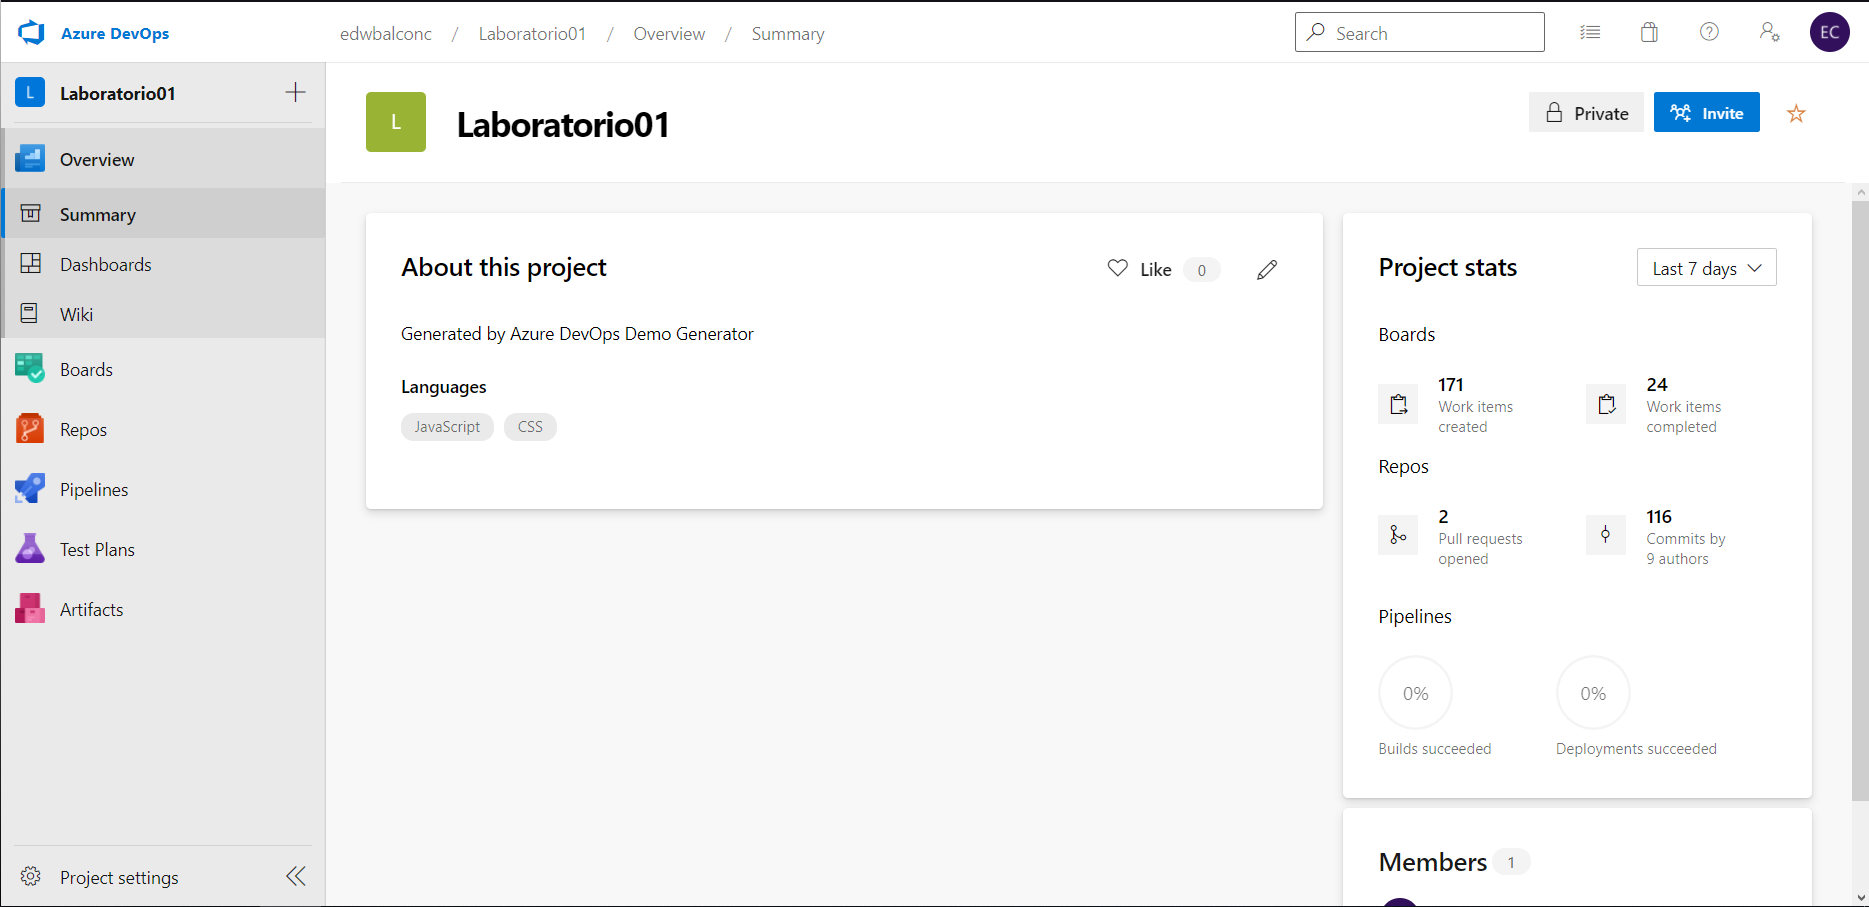
\includegraphics[width=14cm]{./images/1.1} 
	\end{center}
	
\newpage
\textbf{1.2.  Seleccione Test Plans para navegar hasta Test Hub. El centro de pruebas proporciona un lugar central para toda la planificación, ejecución y análisis de pruebas.}

    \begin{center}
		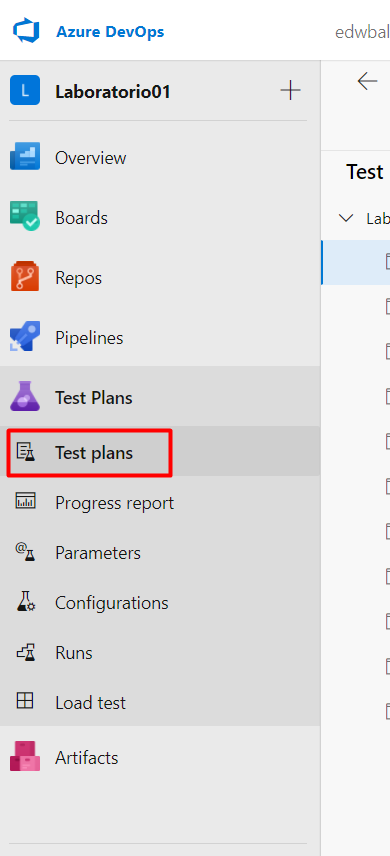
\includegraphics[width=7cm]{./images/1.2} 
	\end{center}
	\newpage
\textbf{1.3. 
En general, cada hito importante de un proyecto debe tener su propio plan de prueba. Dentro de cada plan de prueba hay conjuntos de pruebas, que son colecciones de casos de prueba (y, opcionalmente, otros conjuntos de pruebas) diseñados para validar un elemento de trabajo, como la implementación de una función o la corrección de errores.}

    \begin{center}
		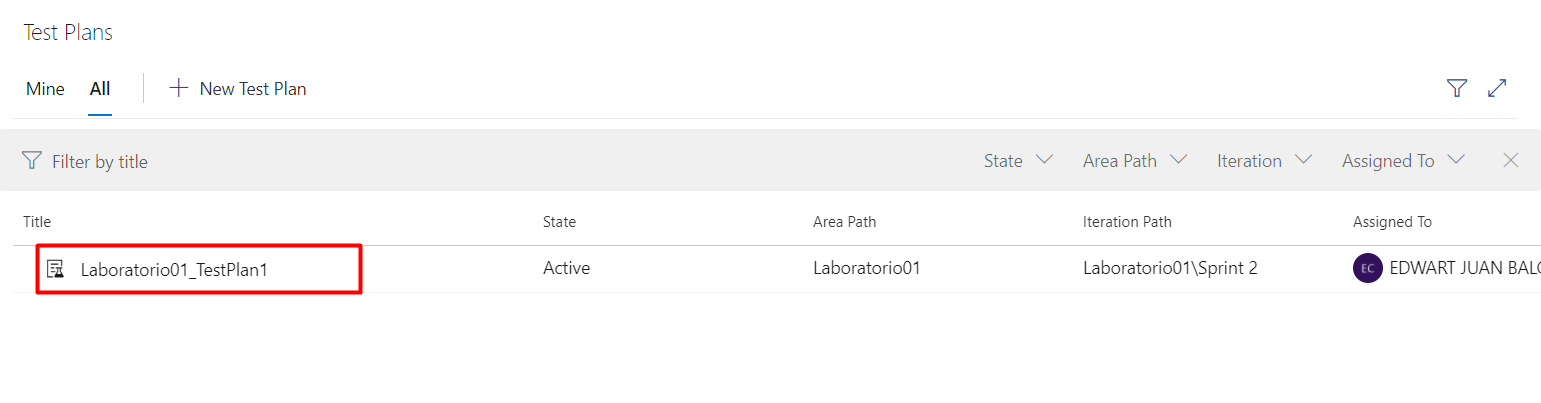
\includegraphics[width=14cm]{./images/1.3} 
	\end{center}
	
\textbf{1.4.  Seleccione el conjunto de pruebas para la historia. Como cliente, me gustaría almacenar los datos de mi tarjeta de crédito de forma segura. .}

    \begin{center}
		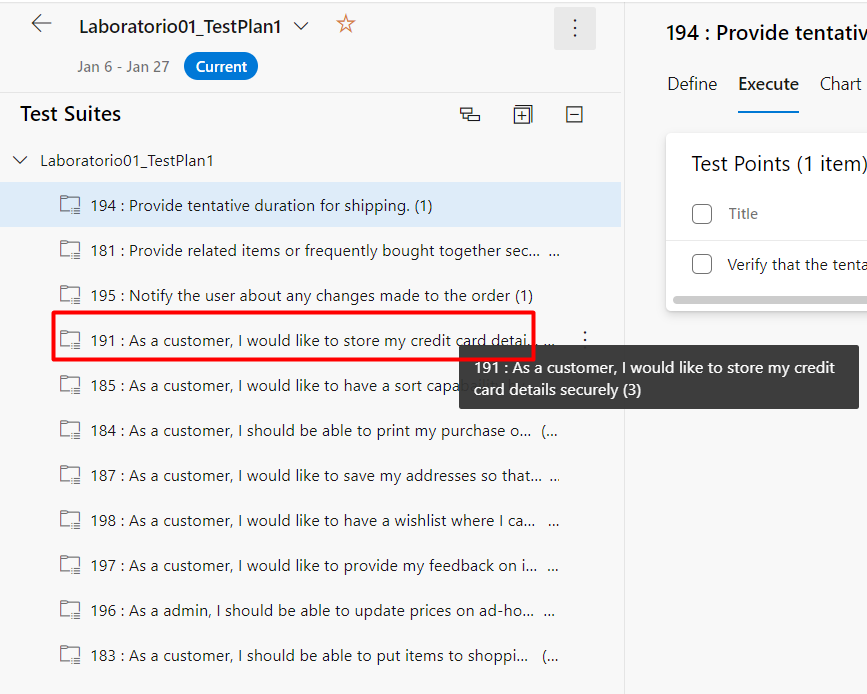
\includegraphics[width=12cm]{./images/1.4} 
	\end{center}
	
\newpage
\textbf{1.5.  En el lado derecho, puede ver que este conjunto de pruebas tiene tres casos de prueba diseñados para confirmar el comportamiento esperado de la implementación de la función. Haga doble clic en Verificar que el usuario pueda guardar el caso de prueba de detalles de su tarjeta de crédito.}

    \begin{center}
		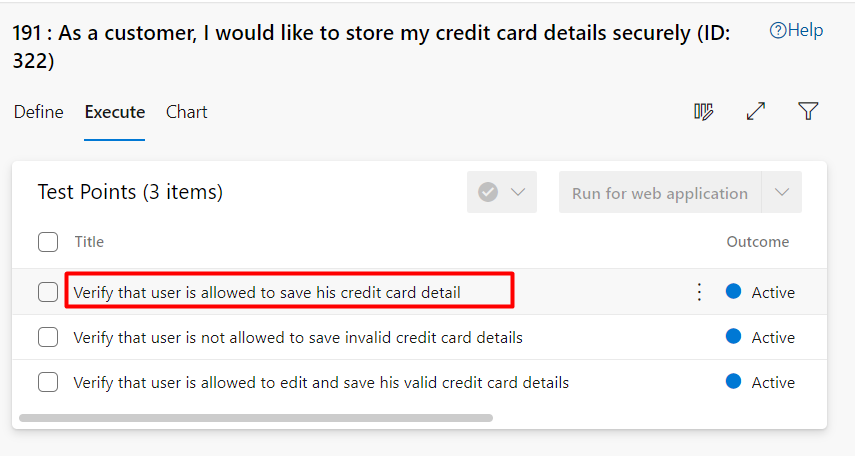
\includegraphics[width=14cm]{./images/1.5} 
	\end{center}
		
\textbf{1.6.Este cuadro de diálogo proporciona toda la información que necesita sobre este caso de prueba. Busque el panel Trabajo relacionado y observe que este caso de prueba está vinculado a la suite a la que pertenece. Haga clic en el elemento de trabajo para navegar hasta él.
}

    \begin{center}
		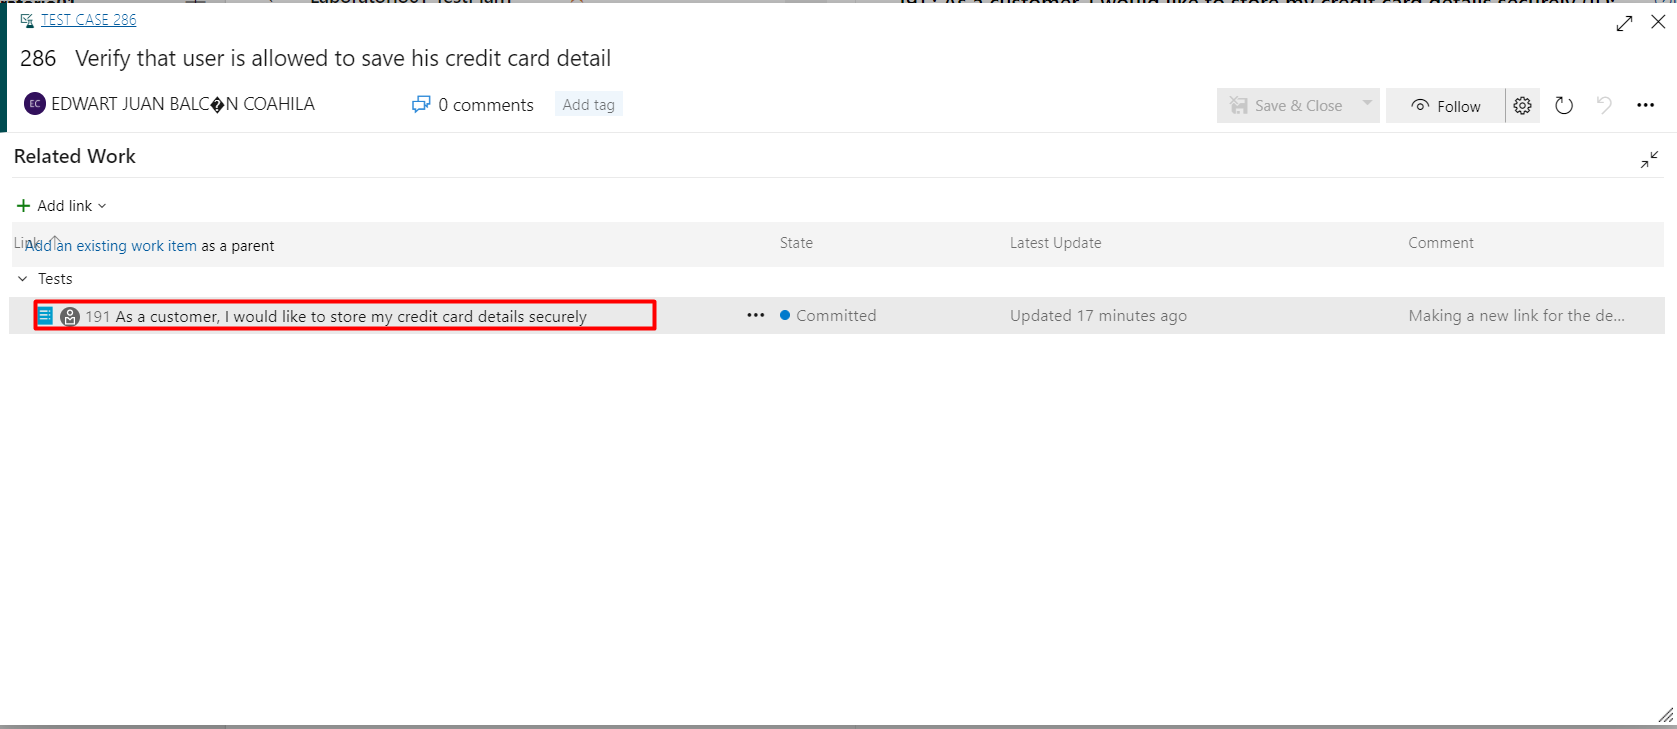
\includegraphics[width=14cm]{./images/1.6} 
	\end{center}
	
\newpage
\textbf{1.7. 
En el conjunto de pruebas, podemos ver todos los elementos de trabajo vinculados, que resultan ser los casos de prueba.}

    \begin{center}
		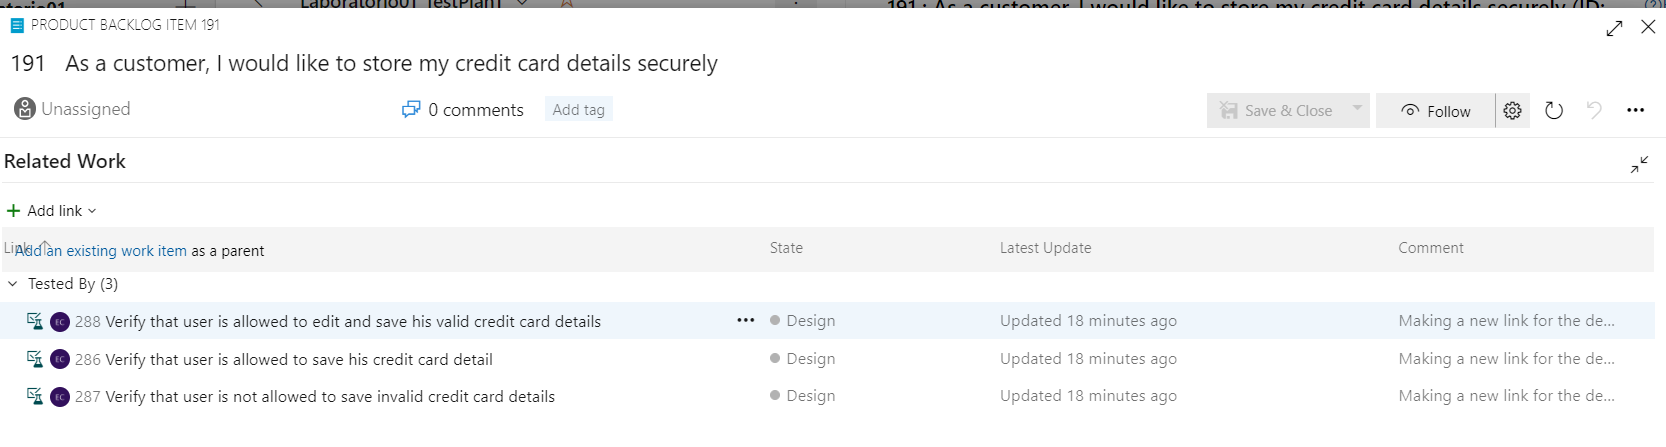
\includegraphics[width=14cm]{./images/1.7} 
	\end{center}
		
\textbf{1.8. Sin embargo, aún no está asociado con la función para la que está diseñado para probar, que podemos vincular ahora. Haga clic en Agregar enlace | Elemento existente.}

    \begin{center}
		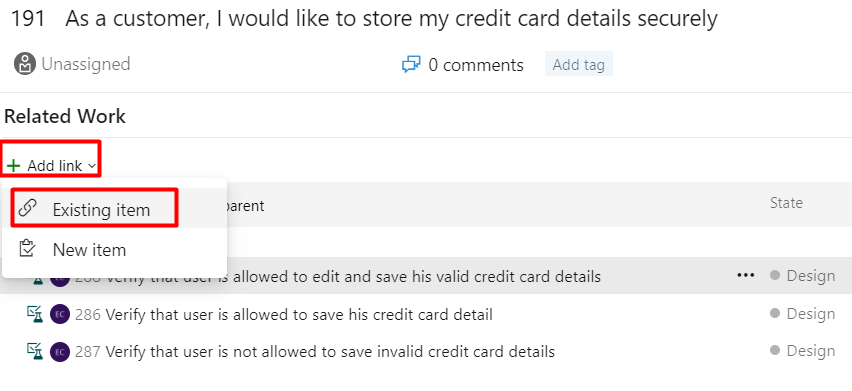
\includegraphics[width=14cm]{./images/1.8} 
	\end{center}
	
\newpage
	
\textbf{1.9. Establezca el tipo de vínculo en Padre y busque "tarjeta de crédito".}

    \begin{center}
		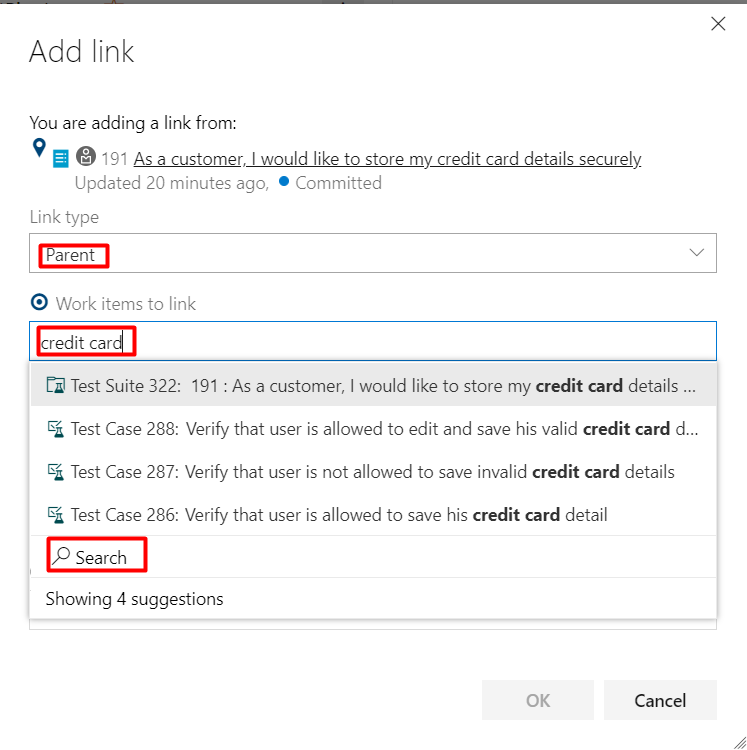
\includegraphics[width=14cm]{./images/1.9} 
	\end{center}
	
\newpage
	
\textbf{1.10. 
Seleccione la función para compra con tarjeta de crédito.}

    \begin{center}
		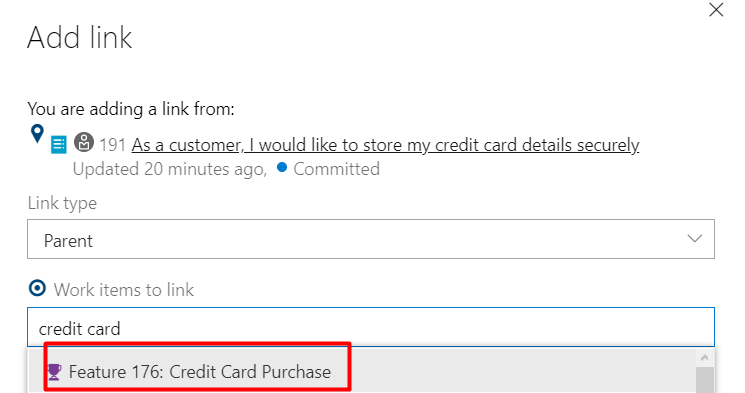
\includegraphics[width=14cm]{./images/1.10} 
	\end{center}

\newpage
	
\textbf{1.11. 
Haga clic en Aceptar.}

    \begin{center}
		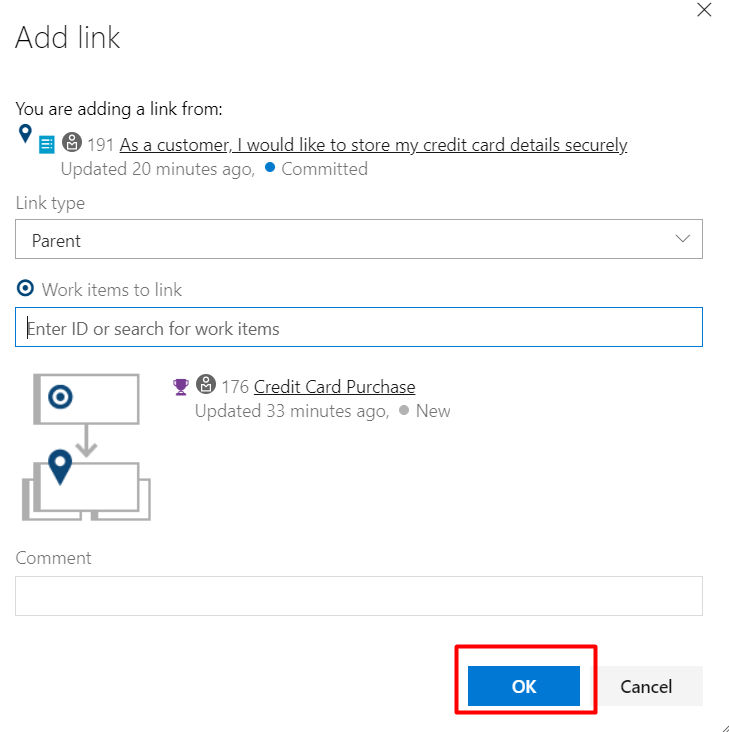
\includegraphics[width=14cm]{./images/1.11} 
	\end{center}

\newpage
	
\textbf{1.12. La función principal ahora está asociada con la suite que la prueba y cualquiera puede navegar entre ellos para ver su relación en relación con los otros elementos de trabajo involucrados.}

    \begin{center}
		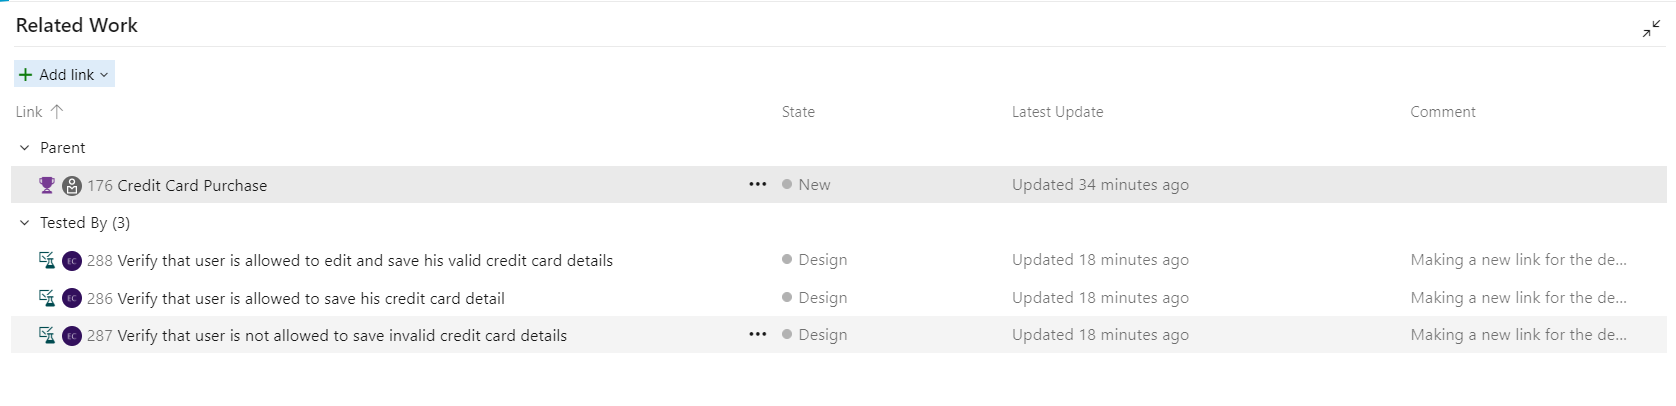
\includegraphics[width=14cm]{./images/1.12} 
	\end{center}

\textbf{1.13. Haga clic en Guardar y cerrar.}

    \begin{center}
		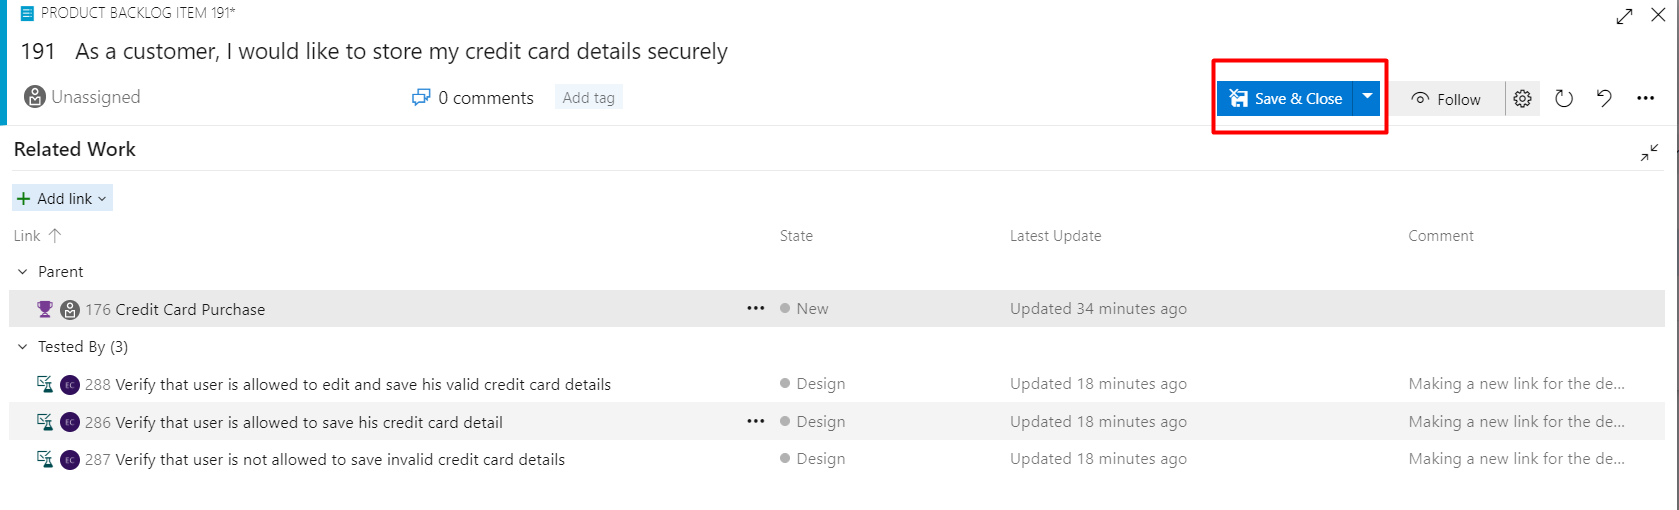
\includegraphics[width=14cm]{./images/1.13} 
	\end{center}
	
\textbf{1.14. Descarte el cuadro de diálogo del caso de prueba original.}

    \begin{center}
		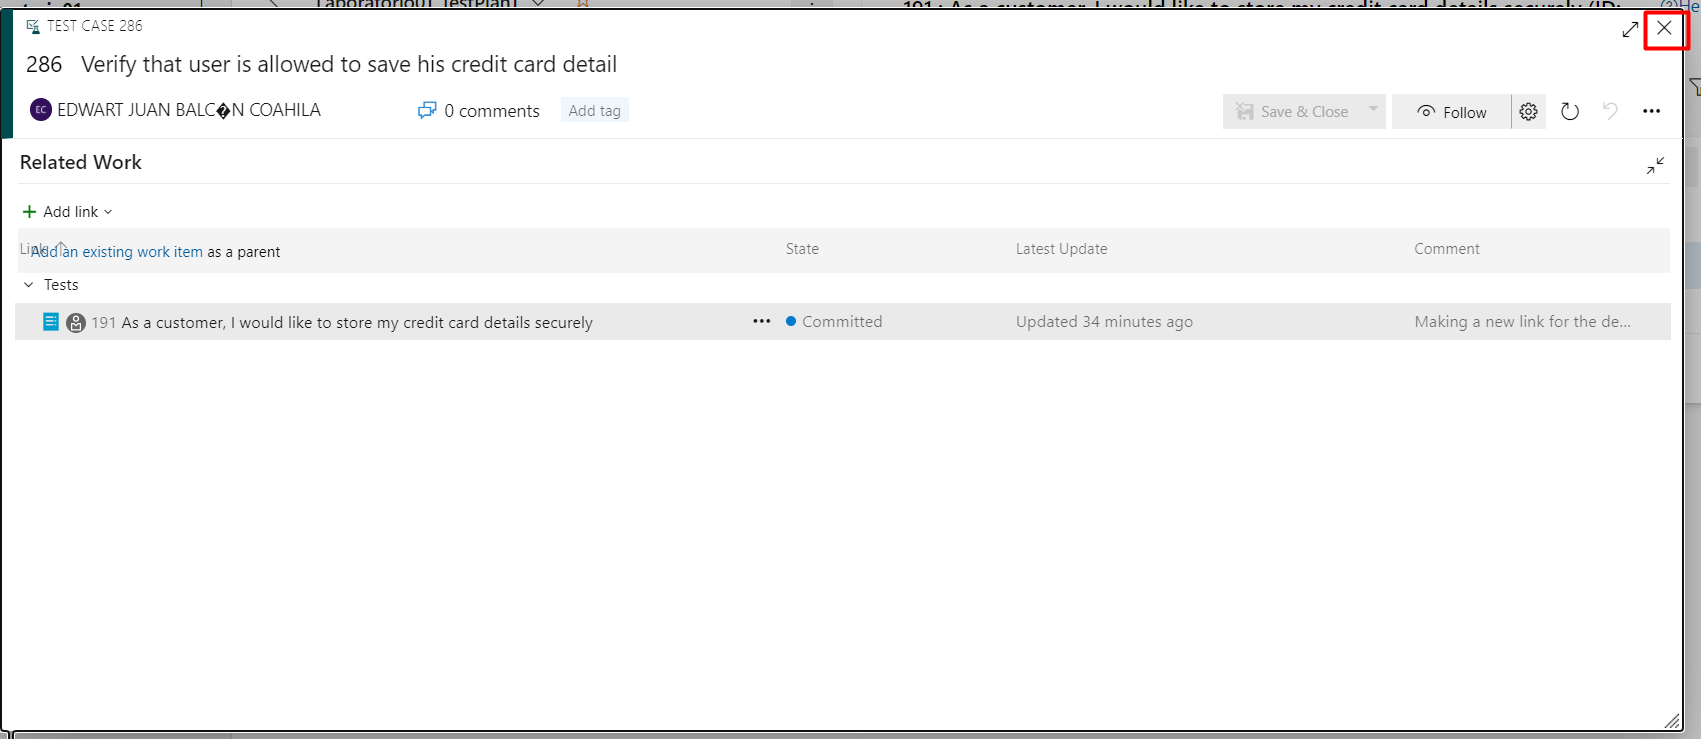
\includegraphics[width=14cm]{./images/1.14} 
	\end{center}


\section{Gestión de pruebas}

\textbf{2.1. Ahora puede ver que el pedido se ha actualizado y que la lista ahora está ordenada por él.}

    \begin{center}
		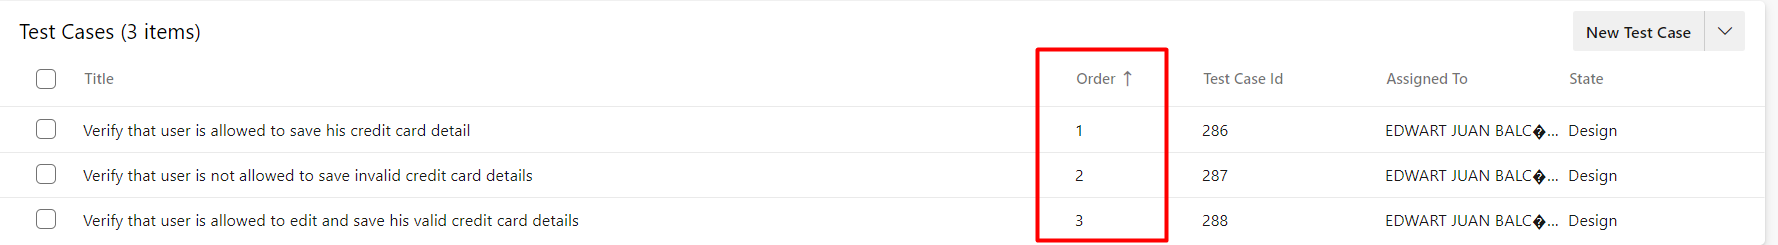
\includegraphics[width=14cm]{./images/2.3} 
	\end{center}
	
\textbf{2.2.  
Seleccione la pestaña Configuraciones.}

    \begin{center}
		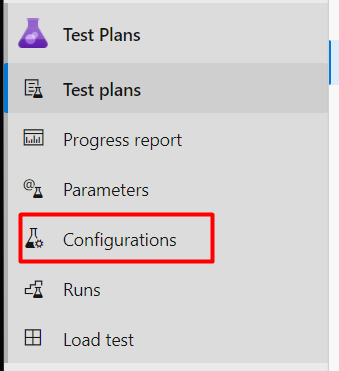
\includegraphics[width=7cm]{./images/2.5} 
	\end{center}
\textbf{2.3. Seleccione la variable del navegador y configúrela en Microsoft Edge.}

    \begin{center}
		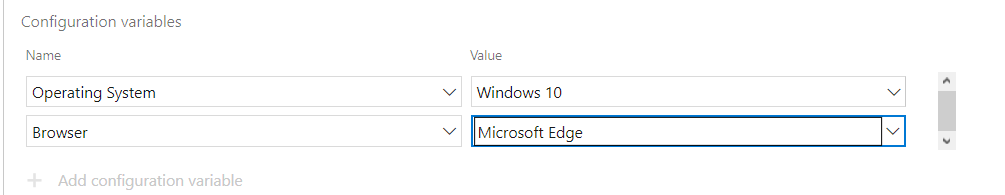
\includegraphics[width=14cm]{./images/2.7}
	\end{center}
		
\newpage
\textbf{2.4.  Haga clic en Guardar para guardar la configuración.}

    \begin{center}
		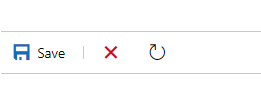
\includegraphics[width=14cm]{./images/2.8} 
	\end{center}
		
\textbf{2.5.Ahora supongamos que el equipo de prueba ha adquirido un iPhone X y quiere agregarlo a la matriz de prueba. Es muy fácil registrar este entorno como una nueva configuración para que los casos de prueba puedan especificarlo. Sin embargo, antes de agregarlo, necesitaremos una opción de sistema operativo para iOS 10. Haga clic en la variable de configuración del sistema operativo.}

    \begin{center}
		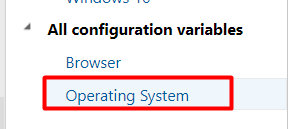
\includegraphics[width=14cm]{./images/2.9} 
	\end{center}
		
\newpage
\textbf{2.6.Haga clic en Agregar nuevo valor y agregue una entrada para iOS 12.}

    \begin{center}
		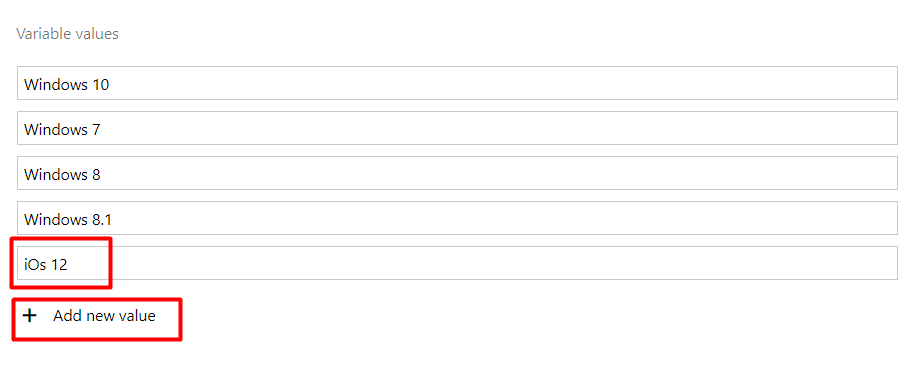
\includegraphics[width=14cm]{./images/2.10} 
	\end{center}
	
\textbf{2.7.Clic en Guardar.}

    \begin{center}
		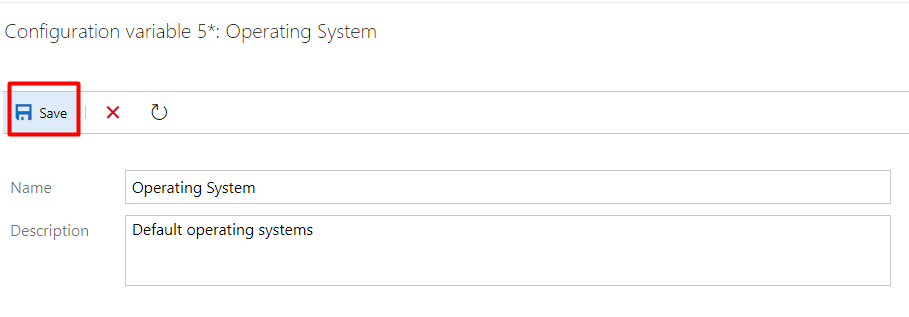
\includegraphics[width=14cm]{./images/2.11} 
	\end{center}
	
	
\newpage
	
\textbf{2.8. Ahora tenemos todo lo que necesitamos para agregar el iPhone X. Haga clic en el menú desplegable Agregar y seleccione Nueva configuración de prueba.}

    \begin{center}
		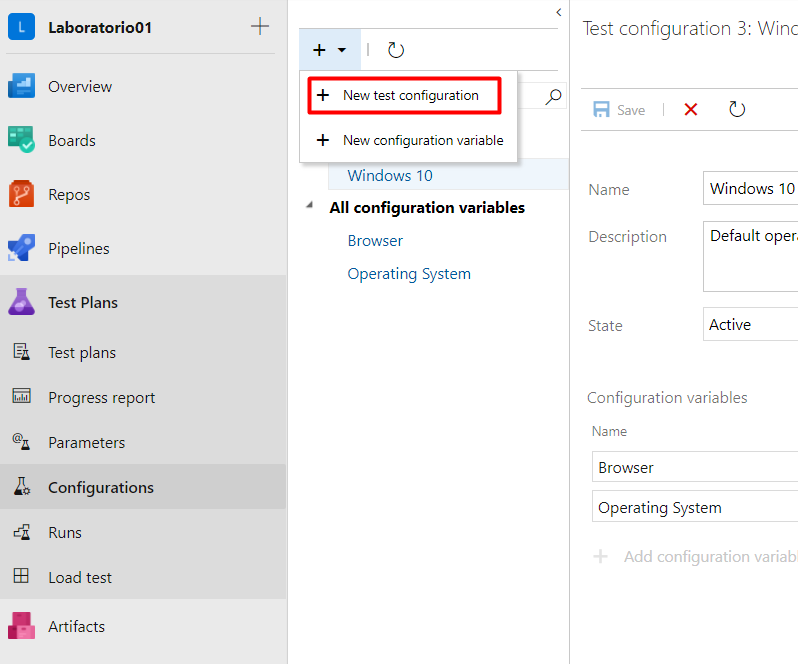
\includegraphics[width=10cm]{./images/2.12} 
	\end{center}
	
\textbf{2.9. Establezca el nombre en "iPhone X".}

    \begin{center}
		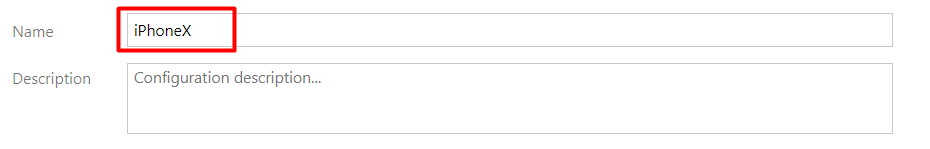
\includegraphics[width=14cm]{./images/2.13} 
	\end{center}
	
\textbf{2.10. Haga clic en Agregar variable de configuración dos veces y configure el navegador en Safari y el sistema operativo en iOS 12.}

    \begin{center}
		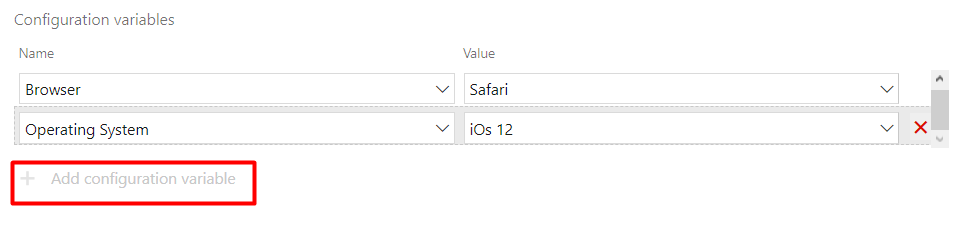
\includegraphics[width=14cm]{./images/2.14} 
	\end{center}
	
\textbf{2.11. Haga clic en Guardar para guardar la nueva configuración.}

    \begin{center}
		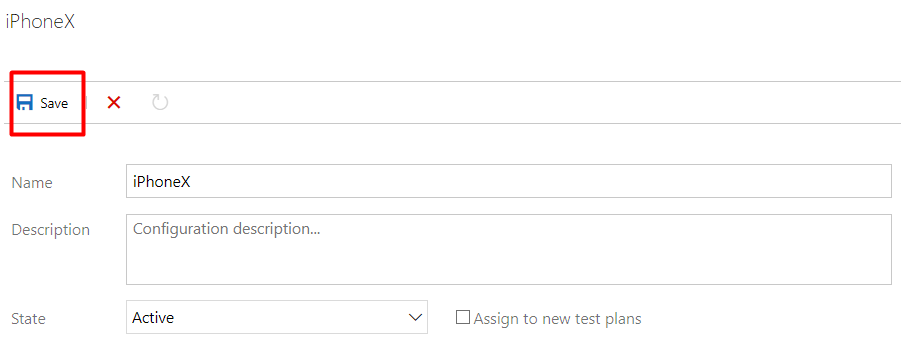
\includegraphics[width=14cm]{./images/2.15} 
	\end{center}
	
\textbf{2.12. Return to the Test Plans tab.}

    \begin{center}
		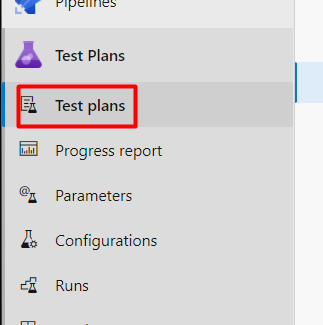
\includegraphics[width=7cm]{./images/2.16} 
	\end{center}
	
\newpage
\textbf{2.13. 
Haga clic en el menú desplegable junto al conjunto de pruebas con el que hemos estado trabajando hasta ahora y seleccione Asignar configuraciones al conjunto de pruebas.}

    \begin{center}
		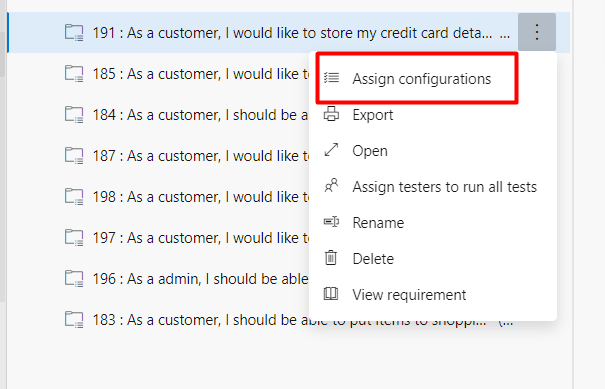
\includegraphics[width=14cm]{./images/2.17} 
	\end{center}
	
\newpage
\textbf{2.14. Marque la opción iPhone X y haga clic en Guardar.}

    \begin{center}
		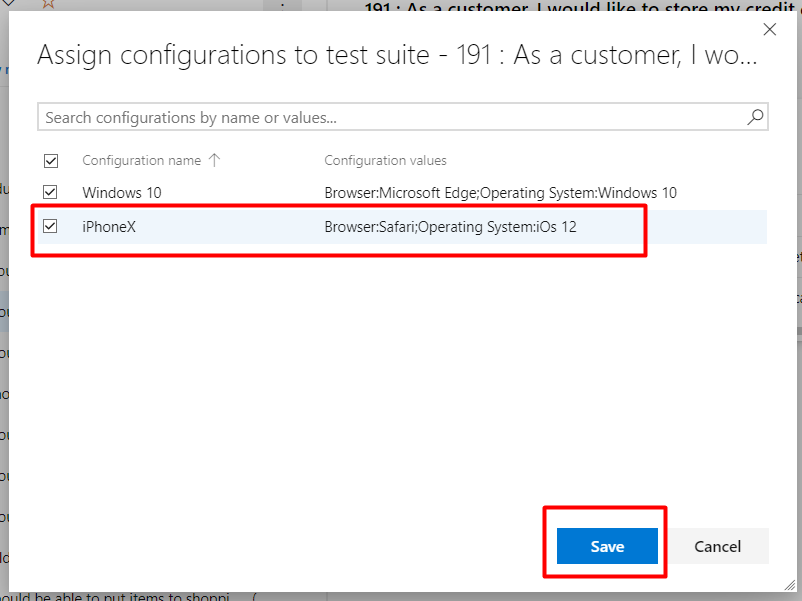
\includegraphics[width=14cm]{./images/2.18} 
	\end{center}
	
\newpage
\textbf{2.15. 
Tenga en cuenta que cada caso de prueba se ha duplicado con una configuración adicional para iPhone X. Ahora cada entorno se puede probar y rastrear por separado.}

    \begin{center}
		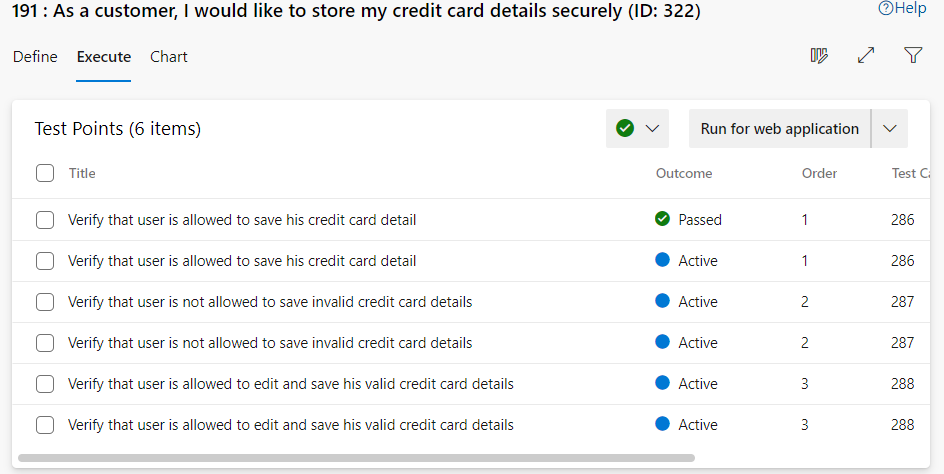
\includegraphics[width=14cm]{./images/2.19} 
	\end{center}
	

\section{
Autoría de pruebas}

\textbf{3.1. Expanda el menú desplegable junto al plan de prueba y seleccione Nueva suite estática.}

    \begin{center}
		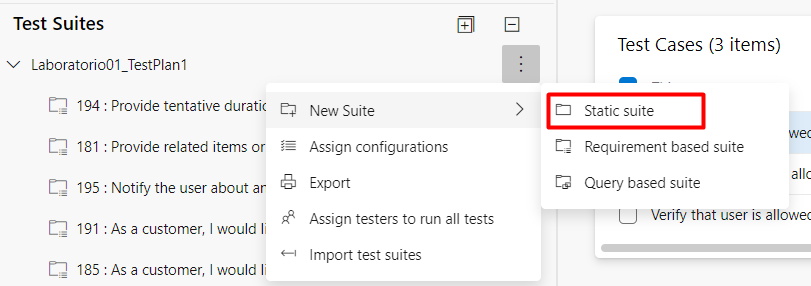
\includegraphics[width=14cm]{./images/3.1} 
	\end{center}
		
\newpage
\textbf{3.2.  
Establezca el nombre de la nueva suite en "Pruebas de envío". Todas estas pruebas se centrarán en la funcionalidad relacionada con el envío. Recuerde que puede compartir fácilmente casos de prueba entre conjuntos, por lo que hay una redundancia mínima cuando hay muchos conjuntos superpuestos.}

    \begin{center}
		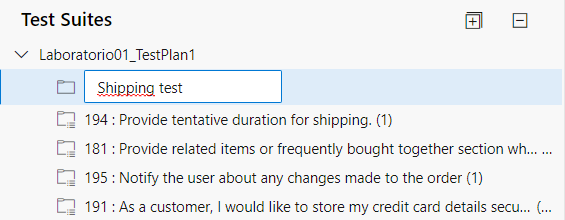
\includegraphics[width=14cm]{./images/3.2} 
	\end{center}
		
\textbf{3.3. Expanda el menú desplegable junto a la suite recién creada y seleccione Nueva suite basada en requisitos.}

    \begin{center}
		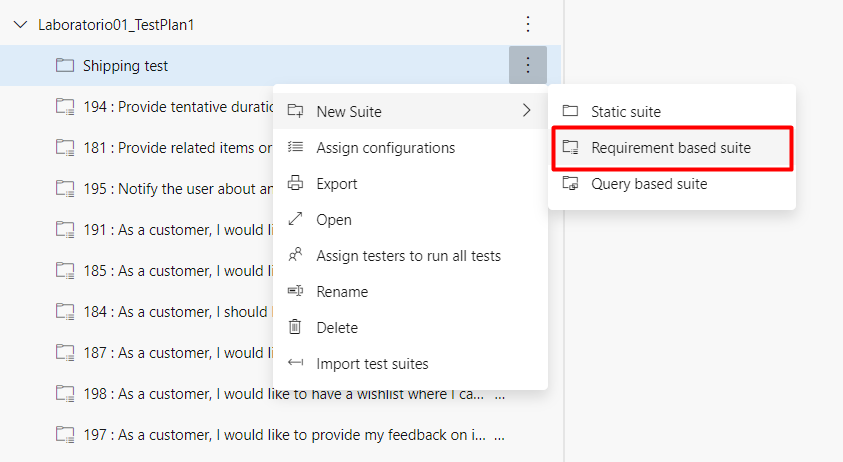
\includegraphics[width=14cm]{./images/3.3} 
	\end{center}
		
\newpage
\textbf{3.4. 
Puede personalizar la consulta utilizada para especificar qué requisitos se recuperan, pero deje los valores predeterminados y haga clic en Ejecutar consulta. }

    \begin{center}
		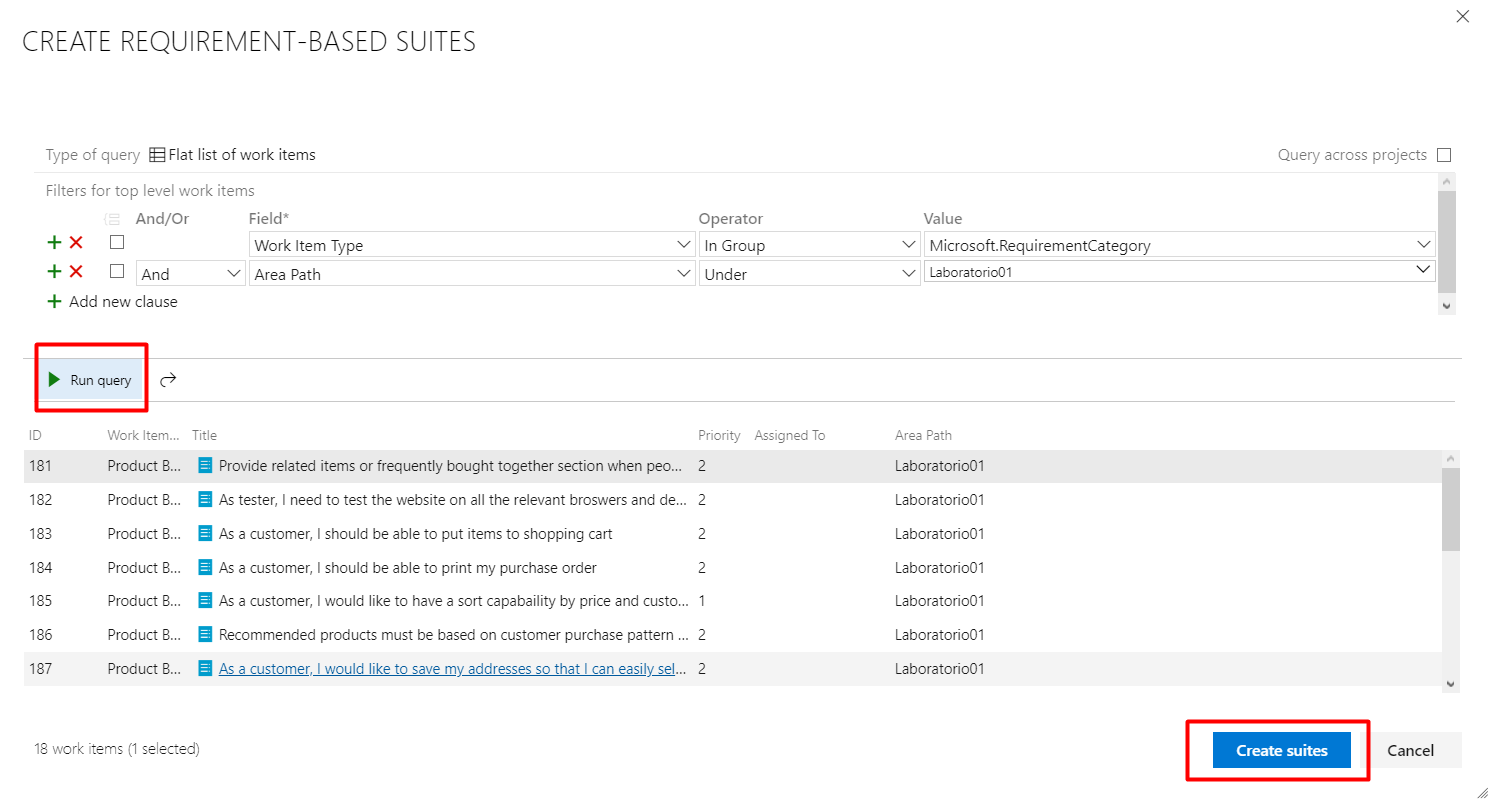
\includegraphics[width=14cm]{./images/3.4} 
	\end{center}
		
\textbf{3.5.Seleccione una de las suites recién creadas, como la asociada con el seguimiento del estado del paquete.}

    \begin{center}
		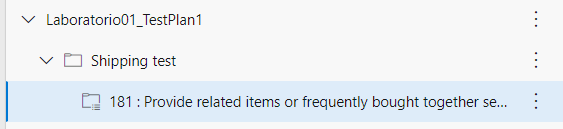
\includegraphics[width=14cm]{./images/3.5} 
	\end{center}
		
\newpage
\textbf{3.6.Si bien puede crear casos de prueba uno a la vez, a veces es más fácil usar un diseño de cuadrícula para agregar rápidamente muchos casos de prueba. En el panel de casos de prueba, seleccione Nuevo | Nuevo caso de prueba usando grid.}

    \begin{center}
		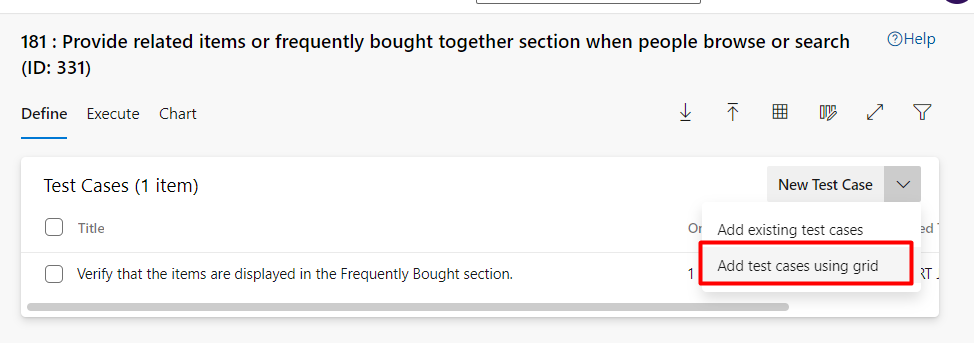
\includegraphics[width=14cm]{./images/3.6} 
	\end{center}
	
	
\end{document}